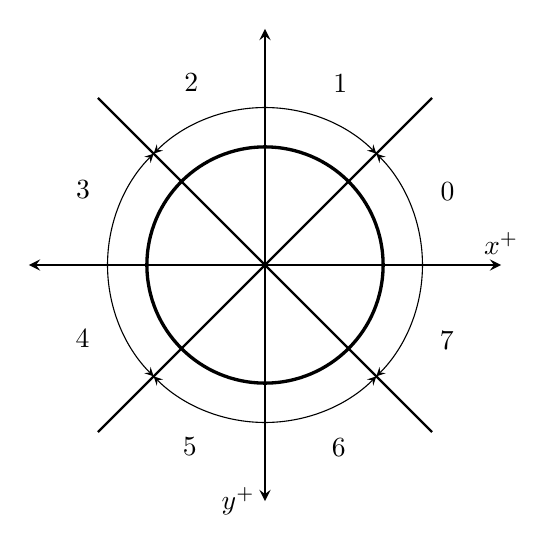
\begin{tikzpicture}[>=stealth]
	\draw [very thick] (0,0) circle (1.5);

	%% Coordinate axes
	\draw [<->,thick] (-3,0) -- (3,0) node [above] {$x^+$};
	\draw [<->,thick] (0,3) -- (0,-3) node [left] {$y^+$};

	%% Diagonals
	\draw [thick] (0,0) +(45:-3) -- (45:3);
	\draw [thick] (0,0) +(135:-3) -- (135:3);

	%% Even arcs
	\foreach \x in {0,1,2,3} {
		\pgfmathmultiply{\x}{90}
		\pgfmathtruncatemacro{\alpha}{\pgfmathresult}
		\draw [->] (0,0) +(0+\alpha:2cm) arc (0+\alpha:45+\alpha:2cm);
		\pgfmathmultiply{\x}{2}
		\pgfmathtruncatemacro{\arclabel}{\pgfmathresult}
		\path (0,0) +(22+\alpha:2.5cm) node {$\arclabel$};
	}

	%% Odd arcs
	\foreach \x in {0,1,2,3} {
		\pgfmathmultiply{\x}{90}
		\pgfmathtruncatemacro{\alpha}{\pgfmathresult}
		\draw [->] (0,0) +(90+\alpha:2cm) arc (90+\alpha:90+\alpha-45:2cm);
		\pgfmathparse{2*\x+1}
		\pgfmathtruncatemacro{\arclabel}{\pgfmathresult}
		\path (0,0) +(67.5+\alpha:2.5cm) node {$\arclabel$};
	}
\end{tikzpicture}
